\chapter{Design of Programming Game}
\label{chap:design-of-game}

\itquote[1mm]{
A game is a problem-solving activity, approached with a playful attitude.
}{J.\,Schell}

%% Terminology + importance.
Students learn programming by solving programming tasks.
% and students spent nearly all the time in the system by solving them.
Therefore, tasks are the key component of a system for learning introductory
programming, and the design of a programming game deserves careful attention.
Similarly to the design of adaptive behavior, a design of a game is also an iterative
process of prototyping and testing new ideas.
Good programming games are a result of many gradual improvements
(\emph{rule of the loop}) \cite{book-of-lenses}.

%...since...
% TODO: terminology: game, task, PS
% NOTE: rule of the loop + strategy: prototyping several ideas, measure
% metrics to see which games work best.

%% Requirements.
The game should allow for tasks practicing all basic
programming concepts, such as sequences of commands, loops, and conditional
statements. % repeat, while, if, if-else, simple tests (comparing)
To enable outer-loop adaptive behavior, multiple diverse tasks practicing the same
concepts are needed, including many tasks using only sequences of commands
without any advanced programming construct.
To support engagement, tasks must be fun and immediately appeal to be
solved.  % TODO: Fix English.
%(TODO: mention how we underestimated the importance of the entertaining tasks in the first prototype)
% (TODO?: other requirements mentioned in the prev. chapters (+REF?)

% TODO: Ideally, mimic and refer to the sections in the chapter on Learning Programming
% (how we incorporated the strategies for easier learning and for motivation)

We have designed a game which is a variation on a robot
on a grid with a space theme, and which uses Blockly (\cref{sec:blockly-games})
for building programs
(\cref{fig:robomission-task2}).
These choices support all main strategies for easier learning of programming
(\cref{sec:strategies-for-easier-learning}),
including
avoiding syntax errors by using block-based programming and
showing a visual output (the grid world).
% and providing short instructions and explanations. % TODO: elaborate?
We combine several strategies to support motivation (\cref{sec:motivation}),
such as appealing game world, entertaining tasks, progressing through levels,
and recommending tasks of optimal difficulty
(adaptivity discussed in \cref{chap:design-of-adaptivity}).
% TODO: target group: Currently, the system primarily targets at children
%  between 10-15 years? (or simply primary school)

\imgW[0.73]{robomission-task2}{%
  Example of a task with the space-themed grid world.}

% NOTE: rule of the loop \cite{book-of-lenses}

\section{Game World}  % Space World
\label{sec:robomission.game-world}

The game world itself should be a pleasure to look at and fun to play with,
even without a specific task to solve \cite{book-of-lenses}.
We have based the game world on a popular choice of a robot on a grid,
using a theme of a spaceship flying through space and collecting diamonds
(\cref{fig:spaceworld}).
% TODO: better word than "popular"?
%% Game elements.
Each field in the \emph{space world} has a background color, which
the spaceship can read and use for decisions (e.g., turning left on red fields).
In addition to the spaceship controlled by the student,
there are the following game objects:
% there are a few other game objects: %, that can reside on one of the fields.
%These are
diamonds, that need to be collected,
large asteroids, that destroy the spaceship if it hits them,
small meteoroids, that can be destroyed,
and wormholes that serve as teleports.

The spaceship starts on the bottom row, and it always moves one row forward
after any action. % towards its final destination (the last row).
% TODO: elaborate / illustrative figure showing a step and a path
In addition to flying and turning, the spaceship can also shoot small meteoroids
(\cref{fig:spaceworld-meteoroids}).
Four basic actions (fly, left, right, shoot) already allows for a
diversity of simple tasks which only practice sequence of commands.
% TODO: limited energy, in order to force thinking about whether to fly or shoot
The spaceship has two sensors, one for the color under the spaceship, and
second for its horizontal position (column index). Having two different sensors allows
for diverse tasks practicing conditions, including testing inequalities, and
potentially also compound conditions.

A novel feature of the game is the default forward movement,
%where turning results in a shift to a neighboring column
%and each action (including turning) are linked with a forward movement.
which results in significantly shorter programs.
For example, to fly around a stone, only two commands are needed % (left, right),
instead of 8 (or 4 if the available commands include
movement in any of the four directions without turning)
(\cref{fig:spaceworld-path}).
% 4: LFFR (e.g., in StarWars game), 8: LFRFFRFL
% TODO: or 4 as a semi-step (single direction OR default movement)
Furthermore, as the spaceship is always facing up, a common left-right
confusion \cite{blockly-10-things} is mitigated.
To avoid too long worlds, we introduced wormholes, that teleport the
spaceship back, to reuse rows multiple times
(\cref{fig:spaceworld-wormholes}).
% (more possible remedies available options available)


%\item movement -- always 1 row forward ("continuous flight ahead") --
%  advantages:
%  (1) mitigates ubiquitous left-right turning confusion;
%  (2) shorter programs (REF example);
%  disadvantages:
%  (1) this behavior is different than what most users initially expect
%  (2) underutilization of fields (only 1 field in each row and only once)
%      (leading to long worlds).
%\item chosen remedy for the 2nd disadvantage: worm holes
%  % (another possibilities: multiple spaceships, long worlds)

%\begin{itemize}
%\item original version - robot-in-maze, issues:
%  \begin{itemize}
%  \item not flexible and did not allow for a lot of diverse easy tasks,
%  \item which is crucial for adaptive learning system
%  \item unnecessarily long programs for simple ideas (non-elegant programs) (TBA: show comparision)
%  \item non-elegant tasks
%  \item ugly worlds
%  \item not very original and entertaining for kids
%  \end{itemize}
%\item requirements (on the topic/theme/world):
%  \begin{itemize}
%  \item entertaining for children
%  \item allowing to create plenty of diverse (and entertaining) tasks, inluding very simple ones
%  \item programs should be not too verbose
%  \item not limiting adaptability (e.g., story requring a fixed sequence of tasks would be a problem)
%  \item (not limiting another topics later)
%  \end{itemize}
%\item fully observable world
%\item no chance (randomness would complicate evaluation and interpretation
%  of data) (there is still some \emph{surprise} in the game for the players:
%  ``Will my program solve the task or not?'')
%%\item REF to formal grammar for the space world in the next chapter
%\end{itemize}


\begin{figure}[htb]
\centering
\begin{subfigure}[t]{0.31\textwidth}
\centering
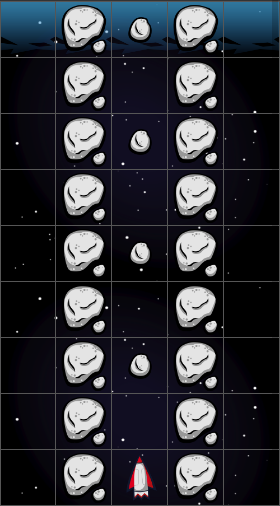
\includegraphics[height=49mm]{img/spaceworld-meteoroids}
\caption{Shootable meteoroids}
\label{fig:spaceworld-meteoroids}
\end{subfigure}
\begin{subfigure}[t]{0.35\textwidth}
\centering
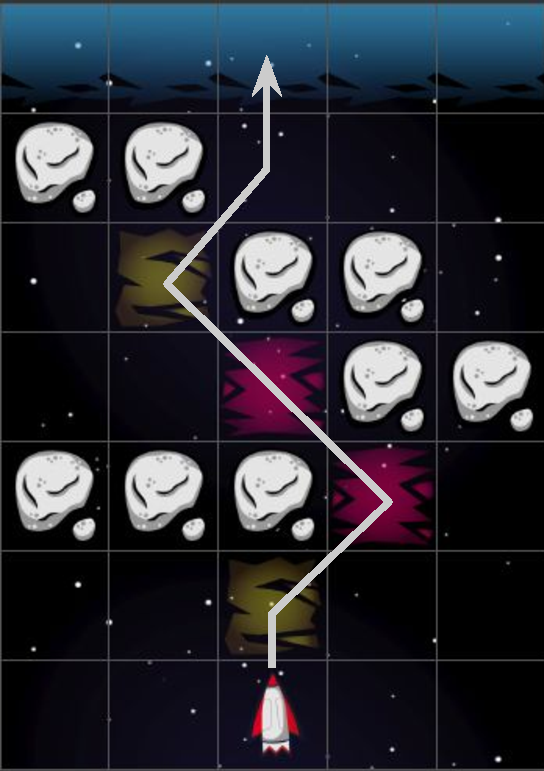
\includegraphics[height=49mm]{img/spaceworld-path}
\caption{Path around asteroids}
\label{fig:spaceworld-path}
\end{subfigure}%
\begin{subfigure}[t]{0.33\textwidth}
\centering
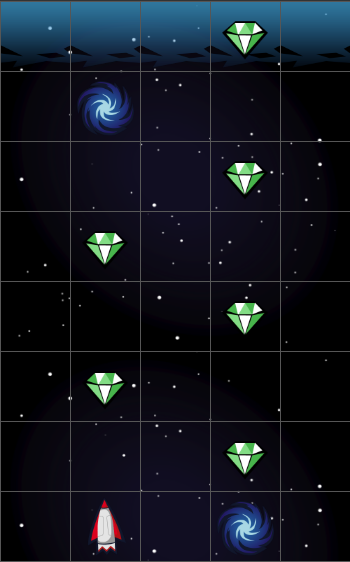
\includegraphics[height=49mm]{img/spaceworld-wormholes}
\caption{Diamonds, wormholes}
\label{fig:spaceworld-wormholes}
\end{subfigure}
\caption{Examples of Space Worlds.}
\label{fig:spaceworld}
\end{figure}


%\imgW{prototype-pits}{Lesson from the first prototype: world must contain
%elements that the program cannot check to enable diverse tasks. As we had a
%natural sensor to check walls, we needed to add pits that could not be checked
%by any sensor.}


\section{Tasks and Programs}
\label{sec:robomission.programs}

Each task asks the student to create a program in Blockly,
that would guide the spaceship safely to the last row,
collecting all diamonds on its way. % (\cref{fig:tasks-solutions}).
% Advantage: very clear and intuitive goal
%Setting of a task consists of a space world description, % as described in the previous section
%optional limits (e.g., maximum length of the program), %, number of shots),
%and available programming blocks (\emph{toolbox}).
Students can execute their current programs as many times
as they need. % wish, and edit them until they solve the task.

%% Blocks.
The set of available blocks is gradually expanding with
increasing level (\cref{sec:level-design}). This \emph{toolbox standardization}
is comfortable for task creators because it is enough to specify
a toolbox only once for all tasks in the same problem set.
% instead of naming all available blocks for each task.
It is also convenient for students since
the available blocks are not changing chaotically with each task.
%- available blocks: depending on the level (sweet spot between chaotically changing toolbox with each task and overloading by all commands from the beginning
% NOTE: blocks: actions (...), sensing (...), repeat, while, if, if-else;
The elementary tasks use only commands for actions (fly, left, right, shoot),
while the more advanced tasks offer \emph{repeat} loop, \emph{while} loop,
\emph{if} and \emph{if-else} statements,
and tests for colors and position.
No special test for the last row is needed since all tasks follow a convention
of coloring the last row by blue color.

%% Programs
To simplify the future learning of a textual programming language,
labels on blocks approximately match Python syntax. % translated to Czech in Czech localization
The most notable exception is the repeat block (\texttt{repeat 5}),
where the Python equivalent (\texttt{for i in range(5)}) is more difficult
to understand for beginners.
% (For details about the blocks and code, see \cref{sec:robocode}.)
% NOTE: in future, this allows for AB experiments
%comparing directly the influence of the text/block environment as done e.g.,
%in the field study in \cite{comparing-blocks-text-weintrop2017}.

%% Limits.
To force students to use loops instead of a long sequence of actions,
a task can specify a \emph{length limit}
on the maximum number of statements in the program.
Limit on the number of statements rather than blocks was chosen in
order to make the limit a smaller number and thus the counting easier.
(Another advantage is that this definition could be used for textual
programming as well.)
To force students to think when they need to shoot, a task can specify
an \emph{energy limit} on the number of shots.

%%% Limits.
%There are two limits that a task can specify.
%The \emph{length} limit defines maximum number of statements
%in the program. Limit on number of statements instead of blocks was chosen in
%order to make the limit a smaller number and thus the counting easier.
%(Another advantage is that this definition could be used for textual
%programming as well.)
%% which is not case for the blocks limit
%This limit forces students to use loops instead of a long sequence of
%actions.
%The \emph{energy} limit controls for the number
%of performed shots. Without this limit, students could always use
%shooting without thinking when it is really needed.


\begin{figure}[htb]
\centering
\begin{subfigure}[t]{0.5\textwidth}
\centering
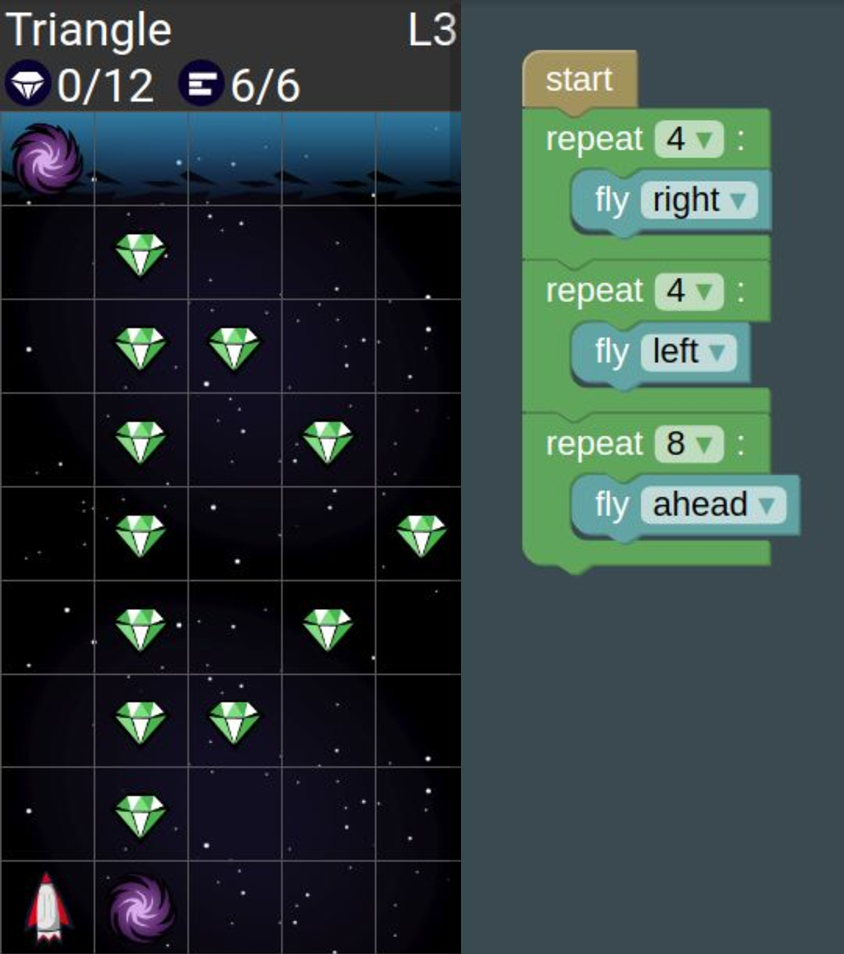
\includegraphics[height=60mm]{img/robomission-task-repeat}
%\caption{Path around asteroids}
%\label{fig:spaceworld-path}
\end{subfigure}%
\begin{subfigure}[t]{0.5\textwidth}
\centering
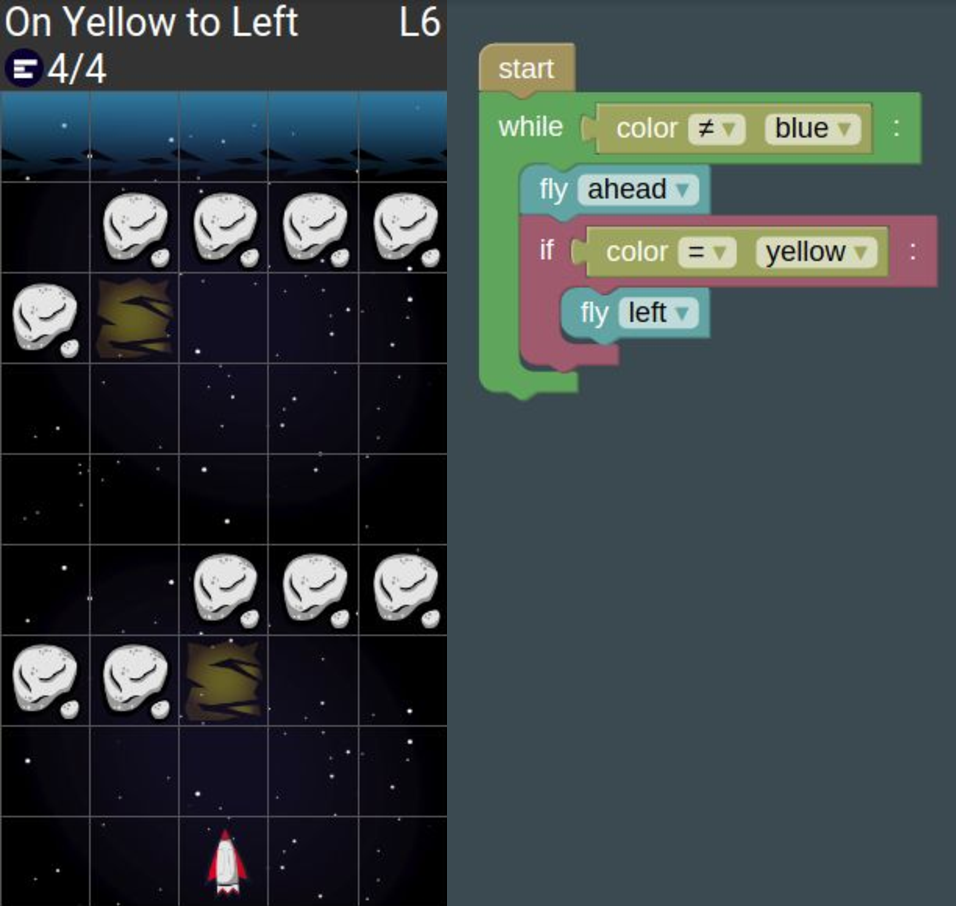
\includegraphics[height=60mm]{img/robomission-task-conditions}
%\caption{Diamonds, wormholes}
%\label{fig:spaceworld-wormholes}
\end{subfigure}
\caption{Examples of tasks and corresponding solutions.}
\label{fig:tasks-solutions}
\end{figure}


\section{Level Design}
\label{sec:level-design}

% TODO: explore and cite: ``level design''

RoboMission contains over 80 tasks divided into nine levels.
% (\cref{fig:robomission-tasks-overview}).
The levels were initially created manually, based on the required blocks
and an estimated difficulty. Later, after some performance data
were collected, we further decomposed them into a two-level
hierarchy to enforce prerequisites between tasks, and we moved
a few tasks into levels that better match their observed
difficulty for students.
% NOTE: But the observed difficulty depends on the context, such as
% the level, the task is presented in.

\imgW[1.0]{robomission-tasks-overview}{%
Tasks overview shows tasks grouped by levels.
The green tasks are solved, the orange task is recommended.
RoboMission contains nine levels, each with about ten tasks.
}


As a motivational element that helps to reinforce the sense of progress,
% OR: to satisfy the need of progress,
students receive credits for each solved task
(\cref{fig:robomission-levels-credits}).
After earning a sufficient number of credits, students progress to next level,
which results in increased difficulty of recommended tasks.

\imgW[1.0]{robomission-levels-credits}{Students earn credits for each solved task.}


\section{Instructions and Explanations}
\label{sec:game.explanations}

Clear hints at appropriate moments
is another strategy to support learning
% OR: to make the learning easier
(\cref{sec:instructions-and-hints}).
We combine simple adaptive instructions and reflexive post-event explanations.
When a student encounters a new programming concept or a game element
for the first time, the system displays a short instruction
(\cref{fig:robomission-mini-instruction}).
% NOTE: They are adaptive in the way that they only show the first time student encounter
% the concept.

\imgW[0.81]{robomission-mini-instruction}{A mini-instruction for a new game concept.}

The system also provides short explanations after each unsuccessful execution,
describing why the task was not solved,
e.g., some diamonds were not collected,
or the spaceship has not reached the final row
(\cref{fig:robomission-mini-explanation}).
% NOTE: simple inner-loop reflexive agent

\imgW[0.81]{robomission-mini-explanation}{A mini-explanation of an unsuccessful attempt.}
%\imgW{prototype-instructions}{Instructions in the first prototype. Nobody was reading them. Most people even did not notice there are any instructions.}

\section{Game Editor}  % OR: task editor?
\label{sec:robomission.task-editor}

The online Game Editor (\cref{fig:game-editor})
helps to create new tasks easily.
In the editor, the author of a task can immediately see a visualization of the
space world,
test a solution in either Blockly or its text-based equivalent %(\emph{RoboCode})
(\cref{fig:game-editor-vim}),
and import or export tasks (using a custom Markdown-based format).
%(TODO: mention how inconvenient it was in the first prototype, especially the tokens...)
The editor is public, so even students can create their own new tasks.
%However, there is currently no support for sharing the tasks with other students.
% Which support the need of creativity; + potentially allows to get a lot of tasks into
% the system, which is could be interesting for adaptivity.

% TODO:
%It allows to switch between RoboCode and RoboBlocks anytime. (REF:transformations)

\imgW[0.86]{game-editor}{Game Editor includes a text editor for game world
(bottom right), which uses an intuitive text representation described in
\cref{sec:impl.spaceworld}.}
\imgW[0.86]{game-editor-vim}{In Vim mode, Game Editor allows to perform some complex
modifications, such as replacing all yellow fields on selected rows to red color,
with a single command.}
